%#MAKEINDEX makeindex interim01
\documentclass[10pt,a4j]{ujarticle}

\newcommand{\setcounters}[1] {
  \setcounter{equation}{#1}
  \setcounter{figure}{#1}
  \setcounter{table}{#1}
}

\newcommand{\unit}[1] {
  \hspace{1mm}\mathrm{[#1]}
}

\newcommand{\degc} {
  \hspace{1mm}\mathrm{[}{}^\circ\mathrm{C]}
}

\newcommand{\refig}[1]{図\ref{fig::#1}}
\newcommand{\refeq}[1]{式(\ref{eq::#1})}
\newcommand{\reftab}[1]{表\ref{tab::#1}}

\newcommand{\fig}[5] {
  \begin{figure}[#1]
    \begin{center}
      \includegraphics[width=#2\hsize]{#3}
    \end{center}
    \caption{#4}
    \label{fig::#5}
  \end{figure}
}

\makeatletter
\def\eq{\@ifstar\@eq\@@eq}
\def\@eq#1{\begin{equation*}#1\end{equation*}}
\def\@@eq#1#2{\begin{equation}#2\label{eq::#1}\end{equation}}
\makeatother

\newcommand{\diff}[2] {
  \frac{\mathrm{d}#1}{\mathrm{d}#2}
}

\newcommand{\pdiff}[2] {
  \frac{\partial #1}{\partial #2}
}


\newcommand{\ddt}[2][1] {
  \ifnum #1 < 2
    \frac{\mathrm{d}#2}{\mathrm{d}t}
  \else
    \frac{\mathrm{d}^#1#2}{\mathrm{d}t^#1}
  \fi
}

\newcommand{\e}[1] {
  \mathrm{e}^{#1}
}

\newcommand{\lparen}{(}
\catcode `( = \active
\newcommand{(}{\ifmmode\left\lparen\else\lparen\fi}

\newcommand{\rparen}{)}
\catcode `) = \active
\newcommand{)}{\ifmmode\right\rparen\else\rparen\fi}

\newcommand{\bmat}[1] {
  \begin{bmatrix} #1 \end{bmatrix}
}

% -- Package ---------------------------------------------------
\usepackage[dvipdfmx]{graphicx}
\usepackage{amsmath, amssymb}
\usepackage{bm}
\usepackage{fancyhdr}
\usepackage{here}
\usepackage{listings}
\usepackage{multirow}


% -- Margin Config ---------------------------------------------
\setlength{\textheight}{\paperheight}
\setlength{\topmargin}{4.6truemm} % 30mm(=1.0in+4.6mm)
\addtolength{\topmargin}{-\headheight}
\addtolength{\topmargin}{-\headsep}
\addtolength{\textheight}{-60truemm}

\setlength{\textwidth}{\paperwidth}
\setlength{\oddsidemargin}{-0.4truemm} % 25mm(=1.0in-0.4mm)
\setlength{\evensidemargin}{-0.4truemm}
\addtolength{\textwidth}{-50truemm}


% -- Renewcommand ----------------------------------------------
\renewcommand{\theequation}{\arabic{section}.\arabic{equation}}
\renewcommand{\thefigure}{\thesection.\arabic{figure}}
\renewcommand{\thetable}{\thesection.\arabic{table}}
\renewcommand{\lstlistingname}{ソースコード}
\renewcommand{\headrulewidth}{0mm} % fancy
\renewcommand{\labelenumi}{(\arabic{enumi})}


% -- Config for fancy package ----------------------------------
\pagestyle{fancy}
\rhead{\thepage}
\lhead{}
\cfoot{}


% -- Config for package listings -------------------------------
\lstset{
  basicstyle={\ttfamily \small},
  breaklines=true,
  frame=trBL,
  numbers=left,
  numberstyle={\ttfamily \small},
}



\begin{document}
%%%%%%%%%%%%%%%%%%%%%%%%%%%%%%%%%%%%%%%%%%%%%%%%%%%%%%%%%%%%%%%%%%%%%%
\section{物品一覧}
今回の配布品,引継ぎ品,購入品についてそれぞれ,以降の表にまとめる.ただし,購入品について※印がついた部品は,購入してテストした結果,使用しなかったものである.\\

今回ロボットにかかった合計金額は, $\yen 76,786$である.

\begin{table}[h]
	\centering
	\caption{配布品一覧}
	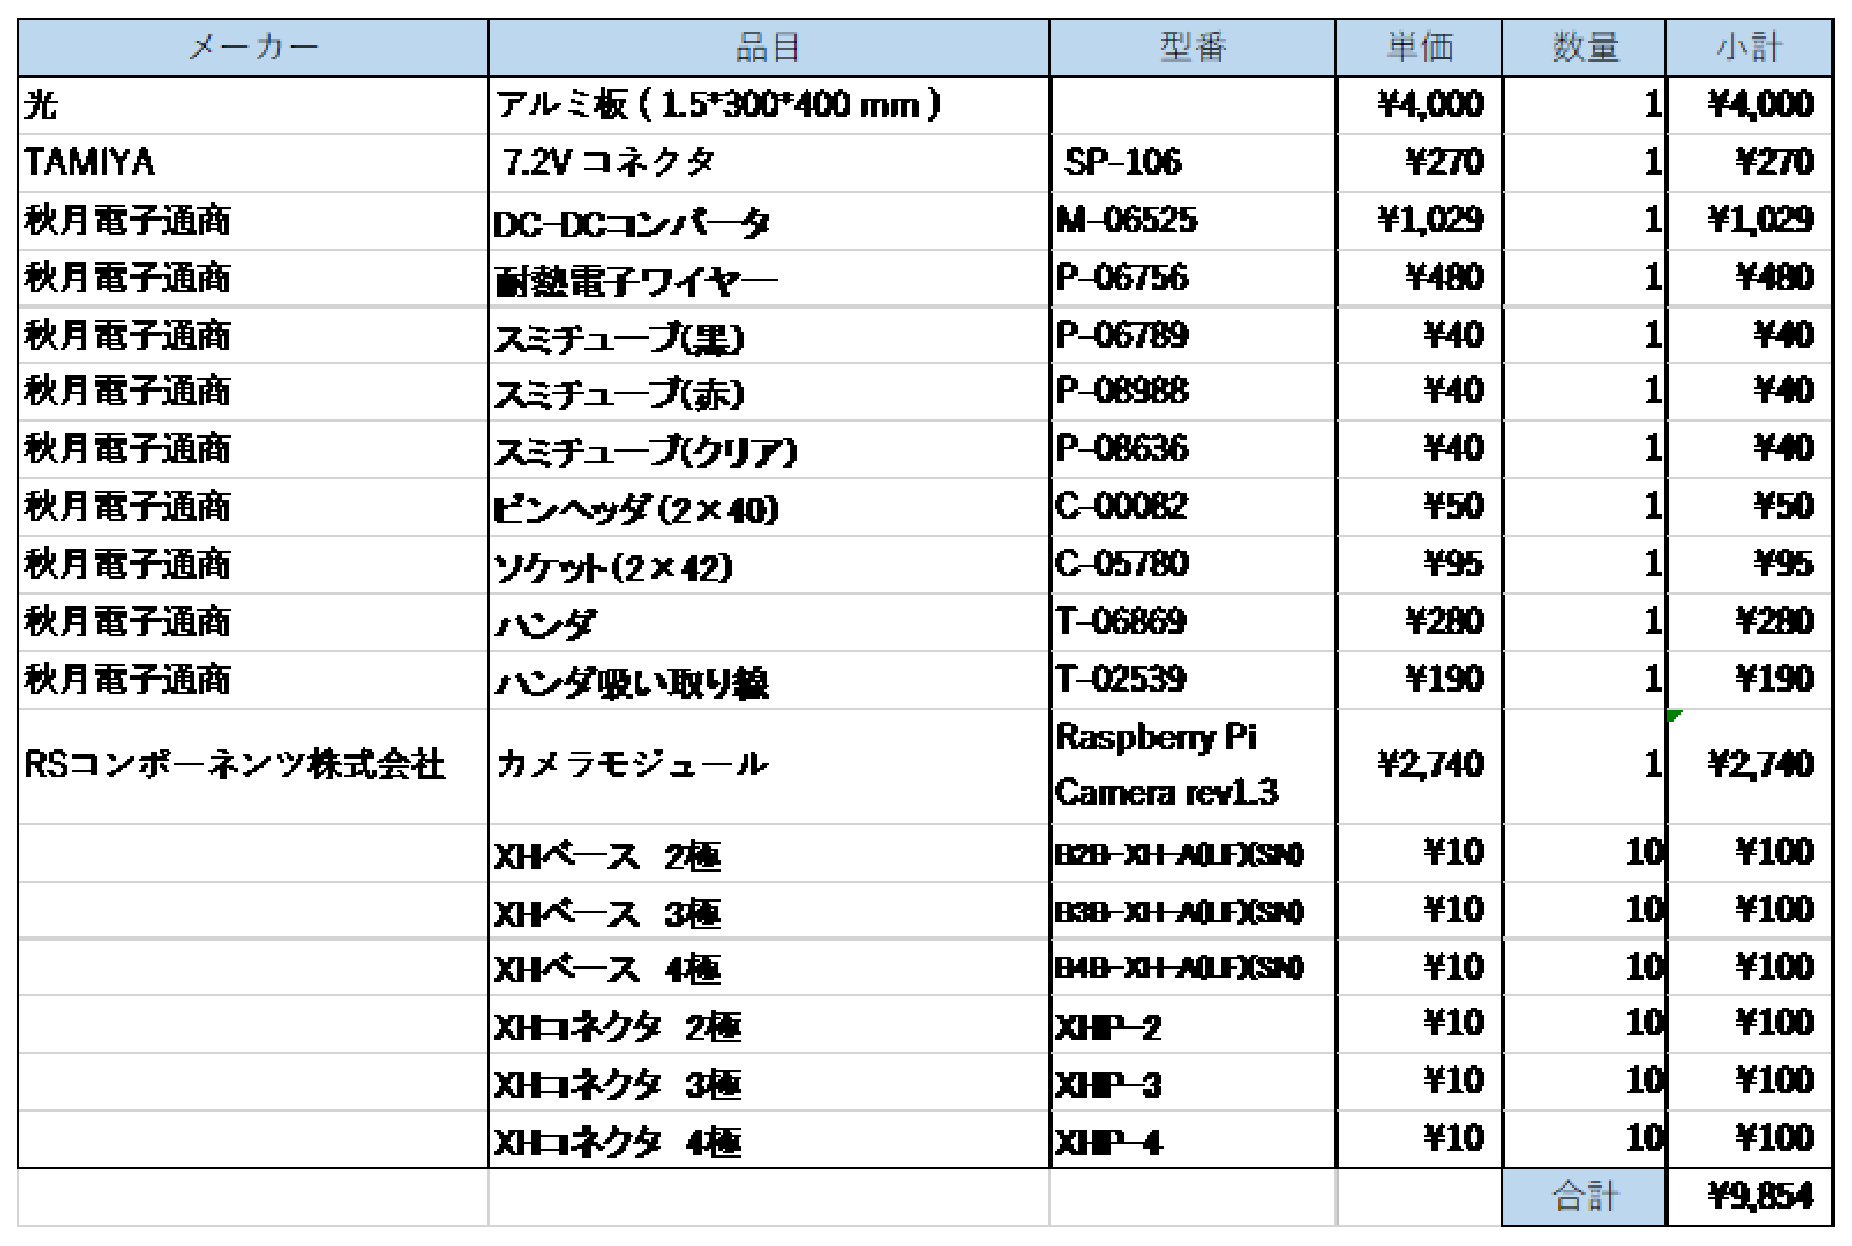
\includegraphics[clip,scale=0.4]{haihu.eps}
    \label{haihu}
\end{table}

\begin{table}[h]
	\centering
	\caption{引継ぎ品一覧}
	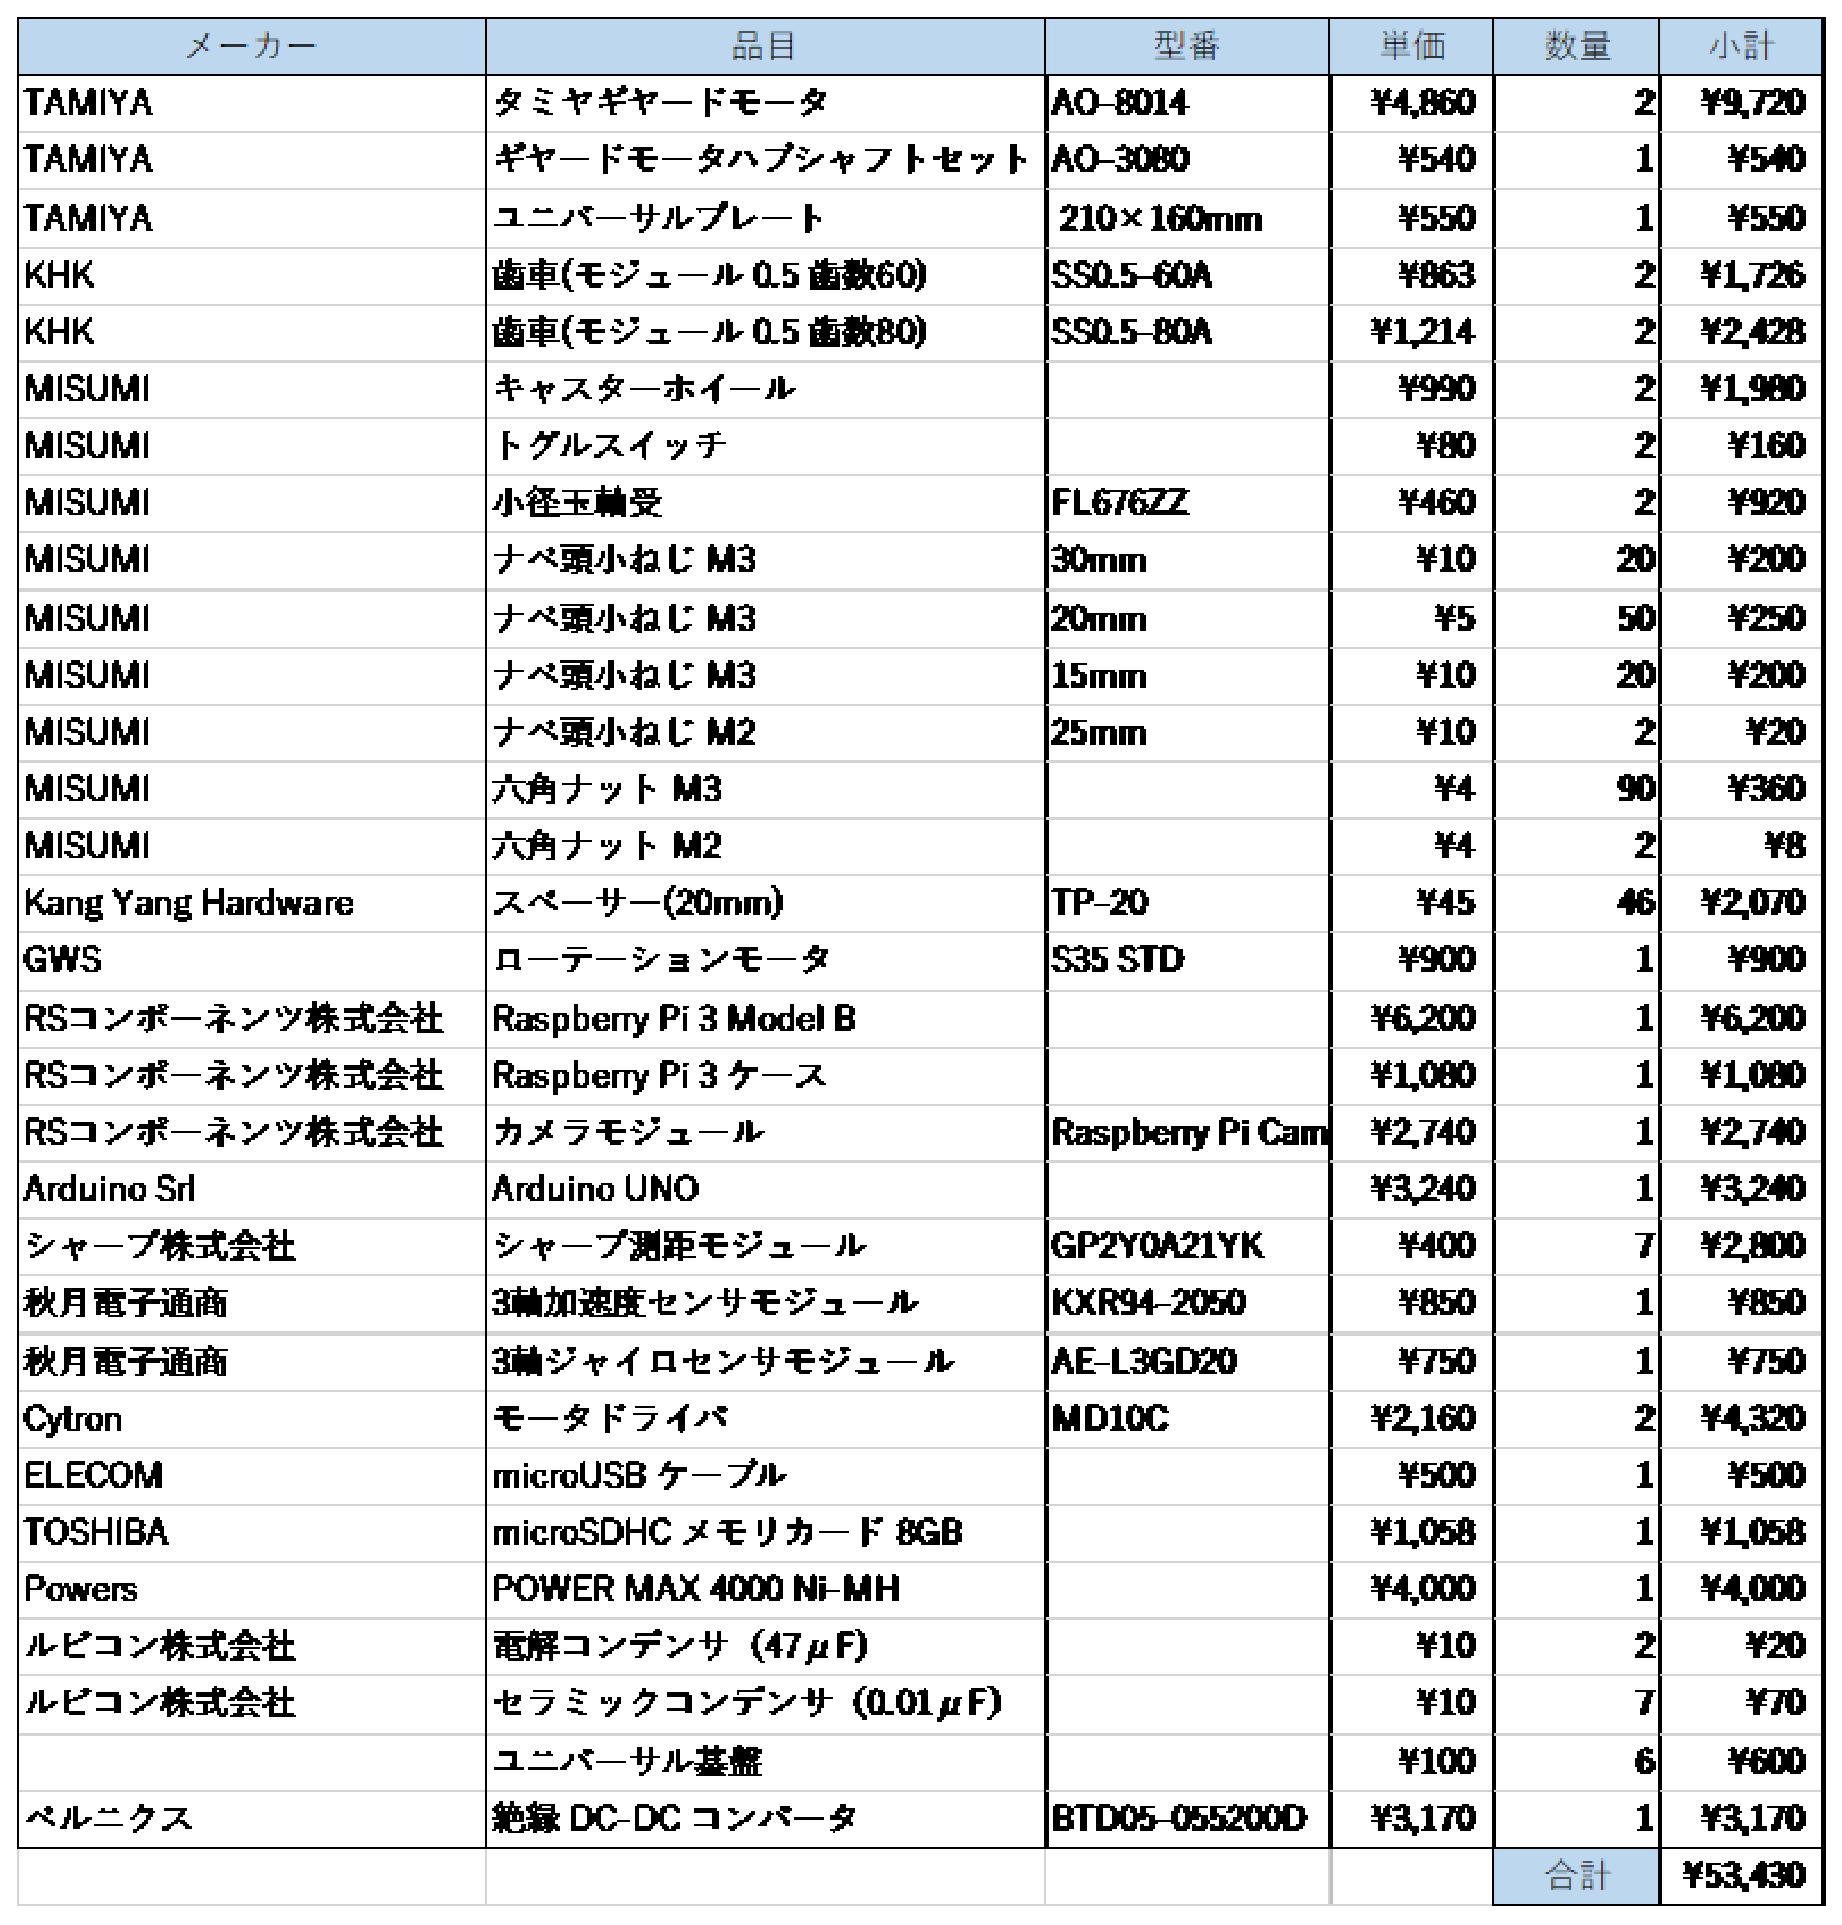
\includegraphics[clip,scale=0.4]{hikitsugi.eps}
 \label{hikitsugi}
\end{table}

\begin{table}[h]
	\centering
	\caption{購入品一覧}
	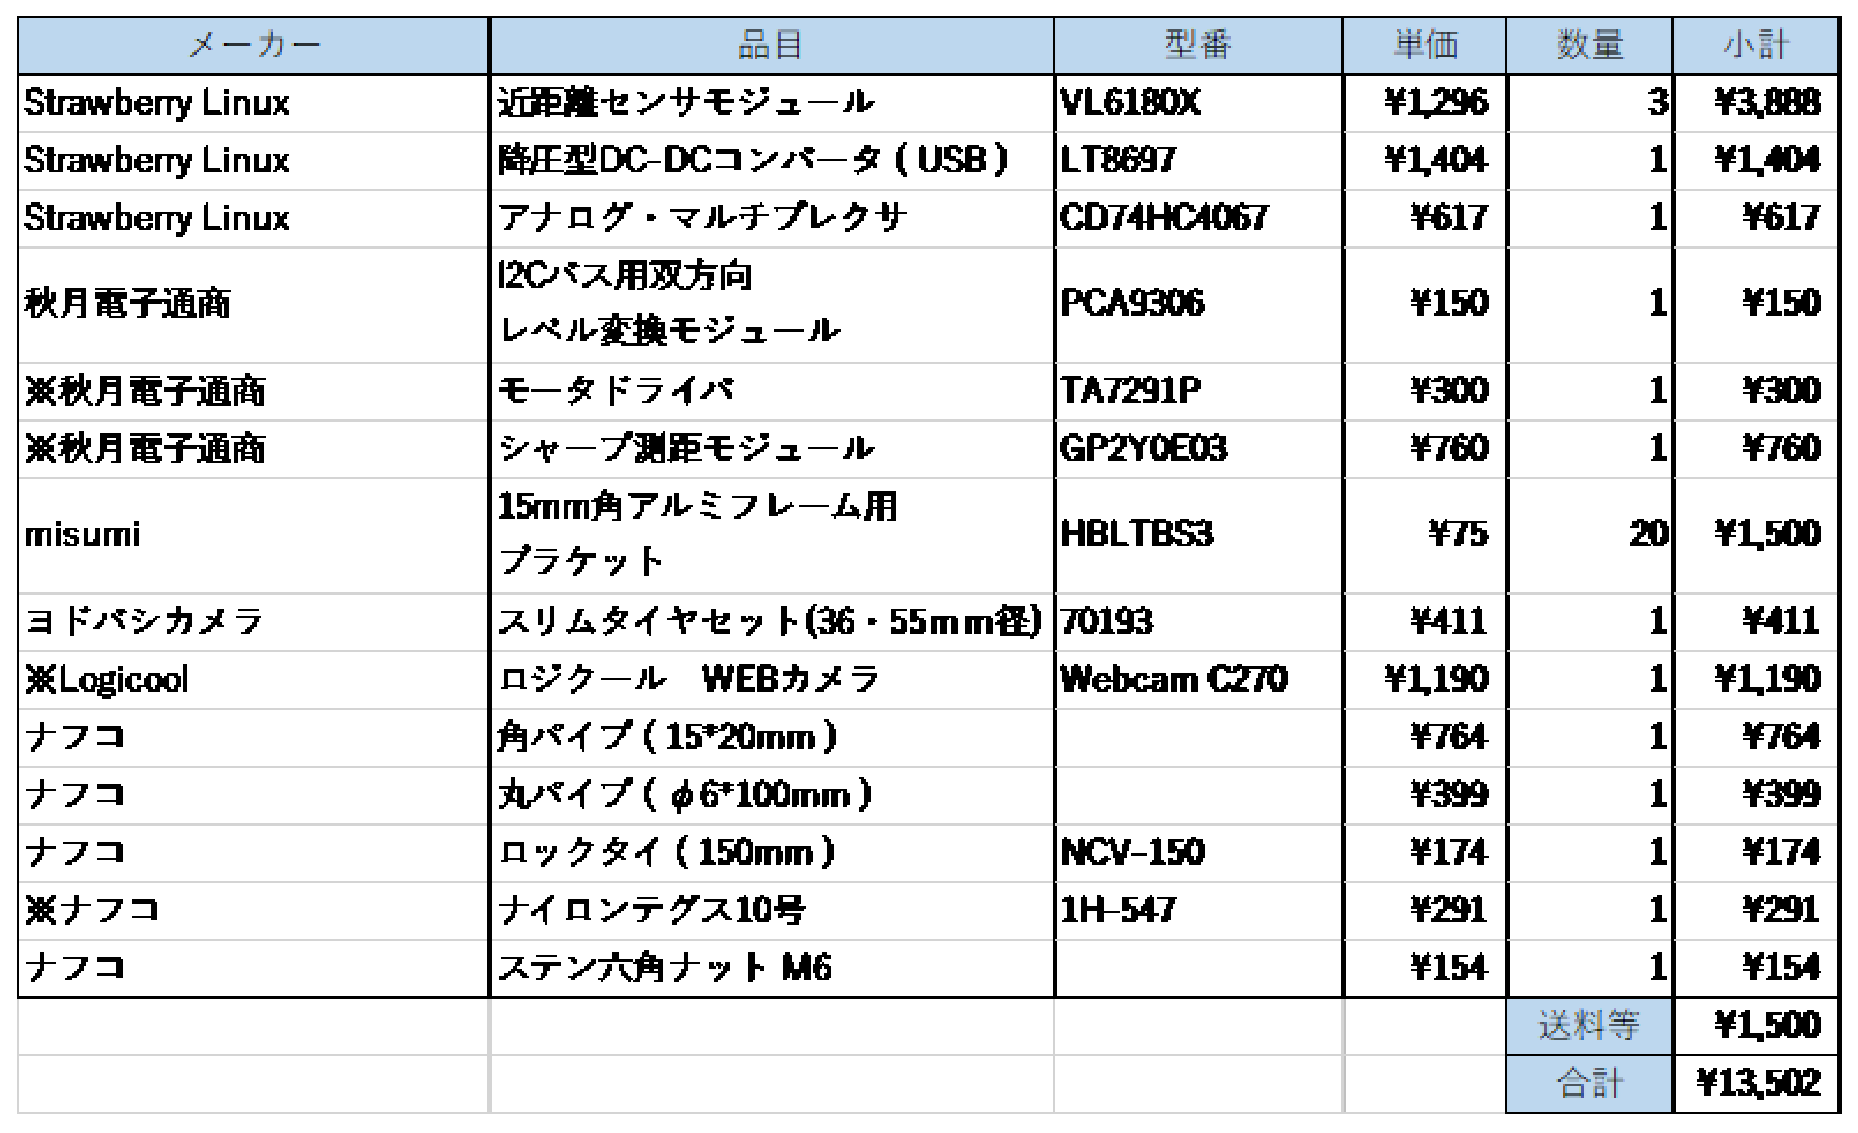
\includegraphics[clip,scale=0.4]{kokunyu.eps}
    \label{kounyu}
\end{table}
%%%%%%%%%%%%%%%%%%%%%%%%%%%%%%%%%%%%%%%%%%%%%%%%%%%%%%%%%%%%%%%%%%%%%%%%%%%%
\end{document}